\documentclass[11pt]{scrartcl}

\usepackage[top=1.5cm]{geometry}
\usepackage{float}
\usepackage{listings}
\usepackage{xcolor}
\usepackage{url}
\usepackage{booktabs}
\usepackage{multicol}
\usepackage{csquotes}
\usepackage{pgfplots}
\usepackage{filecontents}

\usepackage[
    backend=biber,
    style=numeric,
    sorting=none
]{biblatex}

\addbibresource{references/references.bib}

\setlength{\parindent}{0em}
\setlength{\parskip}{0.5em}

\newcommand{\youranswerhere}{[Your answer goes here \ldots]}
\renewcommand{\thesubsection}{\arabic{subsection}}

\lstdefinestyle{dbtsql}{
  language=SQL,
  basicstyle=\small\ttfamily,
  keywordstyle=\color{magenta!75!black},
  stringstyle=\color{green!50!black},
  showspaces=false,
  showstringspaces=false,
  commentstyle=\color{gray}}

\title{
  \textbf{\large Assignment 4} \\
  Index Tuning -- Selection \\
  {\large Database Tuning}}

\author{
  New Group 8 \\
  \large Frauenschuh Florian, 12109584 \\
  \large Lindner Peter, 12101607 \\
  \large Weilert Alexander, 12119653
}

\begin{document}

\maketitle

\paragraph{Notes}

\begin{itemize}
  \item Do not forget to run \lstinline[style=dbtsql]{ANALYZE tablename} after creating or changing a table.
  \item Use \lstinline[style=dbtsql]{EXPLAIN ANALYZE} for the query plans that you display in the report.
\end{itemize}

\subsection*{Experimental Setup}

How do you send the queries to the database? How do you measure the execution time for a sequence of queries?

For our experiments we used the following hardware and software:

\begin{multicols}{2}
  \begin{table}[H]
    \centering
    \begin{tabular}{lc}
      \toprule
      Component & Specs \\
      \midrule
      Processor & i7-13700H 3.7-5.0 GHz \\
      Memory & 32 GiB \\
      \bottomrule
    \end{tabular}
    \caption{Hardware: Dell XPS 15 9530}
    \label{table:hardware}
  \end{table}

  \columnbreak

  \begin{table}[H]
    \centering
    \begin{tabular}{lc}
      \toprule
      Software & Version \\
      \midrule
      OS & Ubuntu 22.04 \\
      Postgres & 2.3.4 \\
      postgresql & 42.7.3 \\
      MariaDB & 10.6.16 \\
      mariadb-java-client & 3.3.3 \\
      Java & 18 \\
      \bottomrule
    \end{tabular}
    \caption{Software}
    \label{table:software_versions}
  \end{table}
\end{multicols}

Postgres was hosted on localhost, on which we also executed our experiments.
The client was implemented in Java and gained access to our databases using the JDBC drivers listed above.

For the queries we used prepared statements, and the performance time was measured by determining the throughput of the
queries in a 60-second time frame.

\subsection*{Clustering B$^+$ Tree Index}

\paragraph{Point Query}

Repeat the following query multiple times with different conditions for \texttt{pubID}.

\begin{lstlisting}[style=dbtsql]
SELECT * FROM Publ WHERE pubID = ?
\end{lstlisting}

Which conditions did you use?

For each query a random existing \texttt{pubID} was chosen.

Show the runtime results and compute the throughput.

\textbf{Executed Queries: } 2003130 \\
\textbf{Queries per Second: } 33385.5

Query plan (for one of the queries):

{\small
\parskip0pt\begin{verbatim}
Index Scan using idx_clustering_pubid on publ  (cost=0.43..8.45 rows=1 width=112)
                                                (actual time=0.051..0.052 rows=1 loops=1)
  Index Cond: ((pubid)::text = 'books/acm/kim95/Kim95'::text)
Planning Time: 0.189 ms
Execution Time: 0.067 ms
\end{verbatim}}

An index scan on the \texttt{pubID} is performed, which make use of the B$^+$ tree index.

\paragraph{Multipoint Query vs. Multipoint Query IN-Predicate -- Low Selectivity}

Repeat the following query multiple times with different conditions for \texttt{booktitle}.

\begin{lstlisting}[style=dbtsql]
SELECT * FROM Publ WHERE booktitle = ?
\end{lstlisting}

\begin{lstlisting}[style=dbtsql]
SELECT * FROM Publ WHERE pubID IN (
    SELECT pubid FROM public.auth WHERE name IN (?, ?, ?))
\end{lstlisting}


Which conditions did you use?

To maintain low selectivity, we are using random non-empty book titles out of the dataset.
Similarly, for the authors, we are choosing three random authors, but do not need to specify the \enquote{non-empty}
condition, since an author is always given.

Show the runtime results and compute the throughput.

\textbf{Multipoint Query}\\
\textbf{Executed Queries: } 153010\\
\textbf{Queries per Second: } 2550.17 \\

\textbf{Multipoint Query IN-Predicate}\\
\textbf{Executed Queries: } 83734\\
\textbf{Queries per Second: } 1395.57

Query plan (for one of the queries):

\textbf{Multipoint Query}
{\small
\parskip0pt\begin{verbatim}
Index Scan using idx_clustering_booktitle on publ  (cost=0.43..14.56 rows=179 width=113)
                                                   (actual time=0.021..0.025 rows=34 loops=1)
  Index Cond: ((booktitle)::text = 'Modern Database Systems'::text)
Planning Time: 0.058 ms
Execution Time: 0.035 ms
\end{verbatim}}

Again, the query plan shows an B$^+$ tree index scan on the \texttt{booktitle}.

\textbf{Multipoint Query IN-Predicate}
{\small
\parskip0pt\begin{verbatim}
Nested Loop  (cost=19.16..628.21 rows=72 width=112)
             (actual time=0.200..4.579 rows=294 loops=1)
  ->  HashAggregate  (cost=18.73..19.45 rows=72 width=23)
                     (actual time=0.171..0.229 rows=294 loops=1)
        Group Key: (auth.pubid)::text
        Batches: 1  Memory Usage: 77kB
        ->  Index Scan using idx_clustering_name on auth
                              (cost=0.43..18.55 rows=72 width=23)
                              (actual time=0.041..0.114 rows=294 loops=1)"
                Index Cond: ((name)::text = ANY
                           ('{""William Kent"",""Alfons Kemper"",""Walid G. Aref""}'::text[]))"
  ->  Index Scan using idx_clustering_pubid on publ
                           (cost=0.43..8.45 rows=1 width=112)
                           (actual time=0.014..0.014 rows=1 loops=294)
        Index Cond: ((pubid)::text = (auth.pubid)::text)
Planning Time: 0.824 ms
Execution Time: 4.625 ms
\end{verbatim}}

This query plan is significantly more complex, as it involves a nested loop and a hash aggregate.
First, an index scan is performed on the \texttt{name} attribute of the \texttt{auth} table, followed by a hash aggregate
operation, due to the use of the \texttt{IN} predicate.
Then, an index scan is performed on the \texttt{pubID} attribute of the \texttt{publ} table.
Finally, the results are joined using a nested loop.

\paragraph{Multipoint Query -- High Selectivity}

Repeat the following query multiple times with different conditions for \texttt{year}.

\begin{lstlisting}[style=dbtsql]
SELECT * FROM Publ WHERE year = ?
\end{lstlisting}

Which conditions did you use?

Same as before, we are using random years from the dataset.

Show the runtime results and compute the throughput.

\textbf{Executed Queries: } 2422\\
\textbf{Queries per Second: } 40.37

Query plan (for one of the queries):

{\small
\parskip0pt\begin{verbatim}
Index Scan using idx_clustering_year on publ  (cost=0.43..2068.83 rows=52823 width=113)
                                              (actual time=0.051..6.806 rows=50803 loops=1)
  Index Cond: ((year)::text = '2000'::text)
Planning Time: 0.054 ms
Execution Time: 7.923 ms
\end{verbatim}}
Similar to the previous query plans, an index scan is performed on the \texttt{year} attribute.

\subsection*{Non-Clustering B$^+$ Tree Index}

\emph{Note:} Make sure the data is not physically ordered by the indexed attributes due to the clustering index that you created before.

\paragraph{Point Query}

Repeat the following query multiple times with different conditions for \texttt{pubID}.

\begin{lstlisting}[style=dbtsql]
SELECT * FROM Publ WHERE pubID = ?
\end{lstlisting}

Which conditions did you use?

For each query a random existing \texttt{pubID} was chosen.

Show the runtime results and compute the throughput.

\textbf{Executed Queries: } 2040997\\
\textbf{Queries per Second: } 34016.62

Query plan (for one of the queries):

{\small
\parskip0pt\begin{verbatim}
Index Scan using idx_clustering_pubid on publ  (cost=0.43..8.45 rows=1 width=112)
                                               (actual time=0.024..0.024 rows=1 loops=1)
  Index Cond: ((pubid)::text = 'books/acm/kim95/Kim95'::text)
Planning Time: 0.052 ms
Execution Time: 0.034 ms
\end{verbatim}}
The query makes use of the B$^+$ tree index on the \texttt{pubID} attribute, just as with the clustering index.

\paragraph{Multipoint Query vs. Multipoint Query IN-Predicate -- Low Selectivity}

Repeat the following query multiple times with different conditions for \texttt{booktitle}.

\begin{lstlisting}[style=dbtsql]
SELECT * FROM Publ WHERE booktitle = ?
\end{lstlisting}

\begin{lstlisting}[style=dbtsql]
SELECT * FROM Publ WHERE pubID IN (
    SELECT pubid FROM public.auth WHERE name IN (?, ?, ?))
\end{lstlisting}


Which conditions did you use?

To maintain low selectivity, we are using random non-empty book titles out of the dataset.
Similarly, for the authors, we are choosing three random authors, but do not need to specify the \enquote{non-empty}
condition, since an author is always given.

Show the runtime results and compute the throughput.

\textbf{Multipoint Query}\\
\textbf{Executed Queries: } 149266\\
\textbf{Queries per Second: } 2487.77 \\

\textbf{Multipoint Query IN-Predicate}\\
\textbf{Executed Queries: } 64079\\
\textbf{Queries per Second: } 1067.98

Query plan (for one of the queries):

\textbf{Multipoint Query}
{\small
\parskip0pt\begin{verbatim}
Index Scan using idx_clustering_booktitle on publ  (cost=0.43..661.90 rows=179 width=112)
                                                    (actual time=0.049..0.051 rows=34 loops=1)
  Index Cond: ((booktitle)::text = 'Modern Database Systems'::text)
Planning Time: 0.172 ms
Execution Time: 0.061 ms

\end{verbatim}}

Again an index scan is performed on the \texttt{booktitle} attribute of the \texttt{publ} table.

\textbf{Multipoint Query IN-Predicate}
{\small
\parskip0pt\begin{verbatim}
Nested Loop  (cost=303.62..938.06 rows=75 width=112) (actual time=1.741..6.267 rows=294 loops=1)
  ->  HashAggregate  (cost=303.19..303.94 rows=75 width=23) (actual time=1.702..1.752 rows=294 loops=1)
        Group Key: (auth.pubid)::text
        Batches: 1  Memory Usage: 77kB
        ->  Bitmap Heap Scan on auth  (cost=13.87..303.00 rows=75 width=23) (actual time=0.105..1.573 rows=294 loops=1)"
              Recheck Cond: ((name)::text = ANY ('{""William Kent"",""Alfons Kemper"",""Walid G. Aref""}'::text[]))"
              Heap Blocks: exact=206
              ->  Bitmap Index Scan on idx_clustering_name  (cost=0.00..13.85 rows=75 width=0) (actual time=0.085..0.085 rows=294 loops=1)"
                    Index Cond: ((name)::text = ANY ('{""William Kent"",""Alfons Kemper"",""Walid G. Aref""}'::text[]))"
  ->  Index Scan using idx_clustering_pubid on publ  (cost=0.43..8.45 rows=1 width=112) (actual time=0.015..0.015 rows=1 loops=294)
        Index Cond: ((pubid)::text = (auth.pubid)::text)
Planning Time: 0.677 ms
Execution Time: 6.316 ms
\end{verbatim}}

First, an index scan with the three chosen authors as in the condition is performed on the name index of the \texttt{auth}
table.
Then, similarly to the clustering index, the hash aggregate operation is performed, followed by an index scan on the
\texttt{pubID} attribute of the \texttt{publ} table.
Finally, the results are joined using a nested loop.

\paragraph{Multipoint Query -- High Selectivity}

Repeat the following query multiple times with different conditions for \texttt{year}.

\begin{lstlisting}[style=dbtsql]
SELECT * FROM Publ WHERE year = ?
\end{lstlisting}

Which conditions did you use?

Same as before, we are using random years from the dataset.

Show the runtime results and compute the throughput.

\textbf{Executed Queries: } 1368\\
\textbf{Queries per Second: } 22.8

Query plan (for one of the queries):

{\small
\parskip0pt\begin{verbatim}
Bitmap Heap Scan on publ  (cost=537.16..23565.35 rows=48095 width=112)
                            (actual time=2.858..51.485 rows=50803 loops=1)
  Recheck Cond: ((year)::text = '2000'::text)
  Heap Blocks: exact=11570
  ->  Bitmap Index Scan on idx_clustering_year  (cost=0.00..525.14 rows=48095 width=0)
                                                (actual time=1.691..1.691 rows=50803 loops=1)
        Index Cond: ((year)::text = '2000'::text)
Planning Time: 0.166 ms
Execution Time: 52.764 ms
\end{verbatim}}

First, a Bitmap Index Scan is performed on the \texttt{year} attribute of the \texttt{publ} table, followed by a Bitmap
Heap Scan.

\subsection*{Non-Clustering Hash Index}

\emph{Note:} Make sure the data is not physically ordered by the indexed attributes due to the clustering index that you created before.

\paragraph{Point Query}

Repeat the following query multiple times with different conditions for \texttt{pubID}.

\begin{lstlisting}[style=dbtsql]
SELECT * FROM Publ WHERE pubID = ?
\end{lstlisting}

Which conditions did you use?

For each query a random existing \texttt{pubID} was chosen.

Show the runtime results and compute the throughput.

\textbf{Executed Queries: } 2618888\\
\textbf{Queries per Second: } 43648.13

Query plan (for one of the queries):

{\small
\parskip0pt\begin{verbatim}
Index Scan using idx_clustering_pubid on publ  (cost=0.00..8.02 rows=1 width=112)
                                                (actual time=0.015..0.016 rows=1 loops=1)
  Index Cond: ((pubid)::text = 'books/acm/kim95/Kim95'::text)
Planning Time: 0.122 ms
Execution Time: 0.025 ms
\end{verbatim}}

For this plan an index scan is again performed on the \texttt{pubID} attribute of the \texttt{publ} table.

\paragraph{Multipoint Query vs. Multipoint Query IN-Predicate -- Low Selectivity}

Repeat the following query multiple times with different conditions for \texttt{booktitle}.

\begin{lstlisting}[style=dbtsql]
SELECT * FROM Publ WHERE booktitle = ?
\end{lstlisting}

\begin{lstlisting}[style=dbtsql]
SELECT * FROM Publ WHERE pubID IN (
    SELECT pubid FROM public.auth WHERE name IN (?, ?, ?))
\end{lstlisting}


Which conditions did you use?

To maintain low selectivity, we are using random non-empty book titles out of the dataset.
Similarly, for the authors, we are choosing three random authors, but do not need to specify the \enquote{non-empty}
condition, since an author is always given.

Show the runtime results and compute the throughput.

\textbf{Multipoint Query}\\
\textbf{Executed Queries: } 137115\\
\textbf{Queries per Second: } 2285.25 \\

\textbf{Multipoint Query IN-Predicate}\\
\textbf{Executed Queries: } 114494\\
\textbf{Queries per Second: } 1908.23

Query plan (for one of the queries):

\textbf{Multipoint Query}
{\small
\parskip0pt\begin{verbatim}
Bitmap Heap Scan on publ  (cost=5.38..672.03 rows=178 width=112) (actual time=0.028..0.038 rows=34 loops=1)
  Recheck Cond: ((booktitle)::text = 'Modern Database Systems'::text)
  Heap Blocks: exact=2
  ->  Bitmap Index Scan on idx_clustering_booktitle  (cost=0.00..5.33 rows=178 width=0) (actual time=0.010..0.010 rows=34 loops=1)
        Index Cond: ((booktitle)::text = 'Modern Database Systems'::text)
Planning Time: 0.209 ms
Execution Time: 0.058 ms
\end{verbatim}}

Unlike the B$^+$ tree index, the hash index performs a Bitmap Index Scan on \texttt{booktitle} and a Bitmap Heap Scan.

\textbf{Multipoint Query IN-Predicate}
{\small
\parskip0pt\begin{verbatim}
Nested Loop  (cost=298.12..892.90 rows=74 width=112) (actual time=1.236..4.378 rows=294 loops=1)
  ->  HashAggregate  (cost=298.12..298.86 rows=74 width=23) (actual time=1.201..1.240 rows=294 loops=1)
        Group Key: (auth.pubid)::text
        Batches: 1  Memory Usage: 77kB
        ->  Bitmap Heap Scan on auth  (cost=12.58..297.94 rows=74 width=23) (actual time=0.038..1.110 rows=294 loops=1)"
              Recheck Cond: ((name)::text = ANY ('{""William Kent"",""Alfons Kemper"",""Walid G. Aref""}'::text[]))"
              Heap Blocks: exact=206
              ->  Bitmap Index Scan on idx_clustering_name  (cost=0.00..12.56 rows=74 width=0) (actual time=0.023..0.023 rows=294 loops=1)"
                    Index Cond: ((name)::text = ANY ('{""William Kent"",""Alfons Kemper"",""Walid G. Aref""}'::text[]))"
  ->  Index Scan using idx_clustering_pubid on publ  (cost=0.00..8.02 rows=1 width=112) (actual time=0.010..0.010 rows=1 loops=294)
        Index Cond: ((pubid)::text = (auth.pubid)::text)
Planning Time: 0.410 ms
Execution Time: 4.417 ms
\end{verbatim}}

A Bitmap Heap Scan is performed on the \texttt{name} attribute of the \texttt{auth} table, followed by hash aggregation.
Then, an index scan is performed on \texttt{pubID} and finally the results are joined using a nested loop.

\paragraph{Multipoint Query -- High Selectivity}

Repeat the following query multiple times with different conditions for \texttt{year}.

\begin{lstlisting}[style=dbtsql]
SELECT * FROM Publ WHERE year = ?
\end{lstlisting}

Which conditions did you use?

Same as before, we are using random years from the dataset.

Show the runtime results and compute the throughput.

\textbf{Executed Queries: } 1318\\
\textbf{Queries per Second: } 21.97

Query plan (for one of the queries):

{\small
\parskip0pt\begin{verbatim}
Bitmap Heap Scan on publ  (cost=1598.36..24675.34 rows=51918 width=113) (actual time=3.368..65.578 rows=50803 loops=1)
  Recheck Cond: ((year)::text = '2000'::text)
  Heap Blocks: exact=12941
  ->  Bitmap Index Scan on idx_clustering_year  (cost=0.00..1585.38 rows=51918 width=0) (actual time=2.102..2.103 rows=50803 loops=1)
        Index Cond: ((year)::text = '2000'::text)
Planning Time: 0.160 ms
Execution Time: 66.916 ms
\end{verbatim}}

Here another Bitmap Index Scan with a Bitmap Heap Scan is performed.

\subsection*{Table Scan}

\emph{Note:} Make sure the data is not physically ordered by the indexed attributes due to the clustering index that you created before.

\paragraph{Point Query}

Repeat the following query multiple times with different conditions for \texttt{pubID}.

\begin{lstlisting}[style=dbtsql]
SELECT * FROM Publ WHERE pubID = ?
\end{lstlisting}

Which conditions did you use?

For each query a random existing \texttt{pubID} was chosen.

Show the runtime results and compute the throughput.

\textbf{Executed Queries: } 2152\\
\textbf{Queries per Second: } 35.87

Query plan (for one of the queries):

{\small
\parskip0pt\begin{verbatim}
Gather  (cost=1000.00..29851.09 rows=1 width=113)
        (actual time=0.226..66.255 rows=1 loops=1)
  Workers Planned: 2
  Workers Launched: 2
  ->  Parallel Seq Scan on publ
        (cost=0.00..28850.99 rows=1 width=113)
        (actual time=24.832..45.490 rows=0 loops=3)
        Filter: ((pubid)::text = 'books/acm/kim95/Kim95'::text)
        Rows Removed by Filter: 411071
Planning Time: 0.627 ms
Execution Time: 66.269 ms
\end{verbatim}}

First, a parallel Seq Scan is performed on the \texttt{publ} table.
Then \texttt{Gather} is used to collect the results from the two parallel workers, from the parallel Seq Scan.
\cite{ParallelQueryDocumentation2024}

\paragraph{Multipoint Query vs. Multipoint Query IN-Predicate -- Low Selectivity}

Repeat the following query multiple times with different conditions for \texttt{booktitle}.

\begin{lstlisting}[style=dbtsql]
SELECT * FROM Publ WHERE booktitle = ?
\end{lstlisting}

\begin{lstlisting}[style=dbtsql]
SELECT * FROM Publ WHERE pubID IN (
    SELECT pubid FROM public.auth WHERE name IN (?, ?, ?))
\end{lstlisting}

Which conditions did you use?

To maintain low selectivity, we are using random non-empty book titles out of the dataset.
Similarly, for the authors, we are choosing three random authors, but do not need to specify the \enquote{non-empty}
condition, since an author is always given.

Show the runtime results and compute the throughput.

\textbf{Multipoint Query}\\
\textbf{Executed Queries: } 1808\\
\textbf{Queries per Second: } 30.13 \\

\textbf{Multipoint Query IN-Predicate}\\
\textbf{Executed Queries: } 342\\
\textbf{Queries per Second: } 5.70

Query plan (for one of the queries):

{\small
\parskip0pt\begin{verbatim}
Gather  (cost=1000.00..29868.99 rows=180 width=112)
        (actual time=0.188..75.361 rows=34 loops=1)
  Workers Planned: 2
  Workers Launched: 2
  ->  Parallel Seq Scan on publ  (cost=0.00..28850.99 rows=75 width=112)
                            (actual time=30.340..54.028 rows=11 loops=3)
        Filter: ((booktitle)::text = 'Modern Database Systems'::text)
        Rows Removed by Filter: 411060
Planning Time: 0.158 ms
Execution Time: 75.373 ms
\end{verbatim}}

Similar to the previous query, a parallel Seq Scan is performed on the \texttt{publ} table, thereafter the results are
gathered from the parallel workers.


{\small
\parskip0pt\begin{verbatim}
Gather  (cost=45542.30..74465.15 rows=73 width=112)
        (actual time=155.433..236.956 rows=294 loops=1)
  Workers Planned: 2
  Workers Launched: 2
  ->  Parallel Hash Semi Join  (cost=44542.30..73457.85 rows=30 width=112)
                               (actual time=141.319..216.325 rows=98 loops=3)
        Hash Cond: ((publ.pubid)::text = (auth.pubid)::text)
        ->  Parallel Seq Scan on publ
                (cost=0.00..27566.39 rows=513839 width=112)
                (actual time=0.383..40.797 rows=411071 loops=3)
        ->  Parallel Hash
                (cost=44541.92..44541.92 rows=30 width=23)
                (actual time=139.036..139.036 rows=98 loops=3)
              Buckets: 1024  Batches: 1  Memory Usage: 72kB
              ->  Parallel Seq Scan on auth
                    (cost=0.00..44541.92 rows=30 width=23)
                        (actual time=89.358..138.993 rows=98 loops=3)
"                    Filter: ((name)::text = ANY
                        ('{""William Kent"",""Alfons Kemper"",""Walid G. Aref""}'::text[]))"
                    Rows Removed by Filter: 1031636
Planning Time: 0.690 ms
Execution Time: 236.986 ms
\end{verbatim}}

For the IN-Predicate query, a Seq Scan is performed on \texttt{auth}.
A parrallel Hash Semi Join joins the results from the parallel Hash, which we used the Seq Scan for, and a parallel Seq
scan on publ.
The results are then gathered from the parallel workers, as before.

\paragraph{Multipoint Query -- High Selectivity}

Repeat the following query multiple times with different conditions for \texttt{year}.

\begin{lstlisting}[style=dbtsql]
SELECT * FROM Publ WHERE year = ?
\end{lstlisting}

Which conditions did you use?

Same as before, we are using random years from the dataset.

Show the runtime results and compute the throughput.

\textbf{Executed Queries: } 1276\\
\textbf{Queries per Second: } 21.27

Query plan (for one of the queries):

{\small
\parskip0pt\begin{verbatim}
Gather  (cost=1000.00..35038.69 rows=51877 width=112)
        (actual time=0.221..77.570 rows=50803 loops=1)
  Workers Planned: 2
  Workers Launched: 2
  ->  Parallel Seq Scan on publ  (cost=0.00..28850.99 rows=21615 width=112)
                                (actual time=0.024..55.584 rows=16934 loops=3)
        Filter: ((year)::text = '2000'::text)
        Rows Removed by Filter: 394137
Planning Time: 0.117 ms
Execution Time: 78.799 ms
\end{verbatim}}

A parallel Seq Scan is performed on the \texttt{publ} table and then the results from the two workers are gathered.

\subsection*{Discussion}

Give the throughput of the query types and index types in queries/second.
\begin{table}[H]
  \centering
  \begin{tabular}{c|c|c|c|c}
    & clustering & non-clust.\ B$^+$ tree & non-clust.\ hash & table scan
      \tabularnewline
    \hline
    point (\texttt{pubID}) & 33385.5 & 34016.62 & 43648.13 & 35.86 \tabularnewline
    \hline
    multipoint (\texttt{booktitle}) & 2550.17 & 2487.77 & 2285.25 & 30.13
      \tabularnewline
    \hline
		multipoint-IN (\texttt{pubID}) & 1395.56 & 1067.98 & 1908.23 & 5.70
      \tabularnewline
		\hline
    multipoint (\texttt{year}) & 40.37 & 22.8 & 21.96 & 21.27
      \tabularnewline
  \end{tabular}
\end{table}

Discuss the runtime results for the different index types and the table scan. Are the results expected? Why (not)?

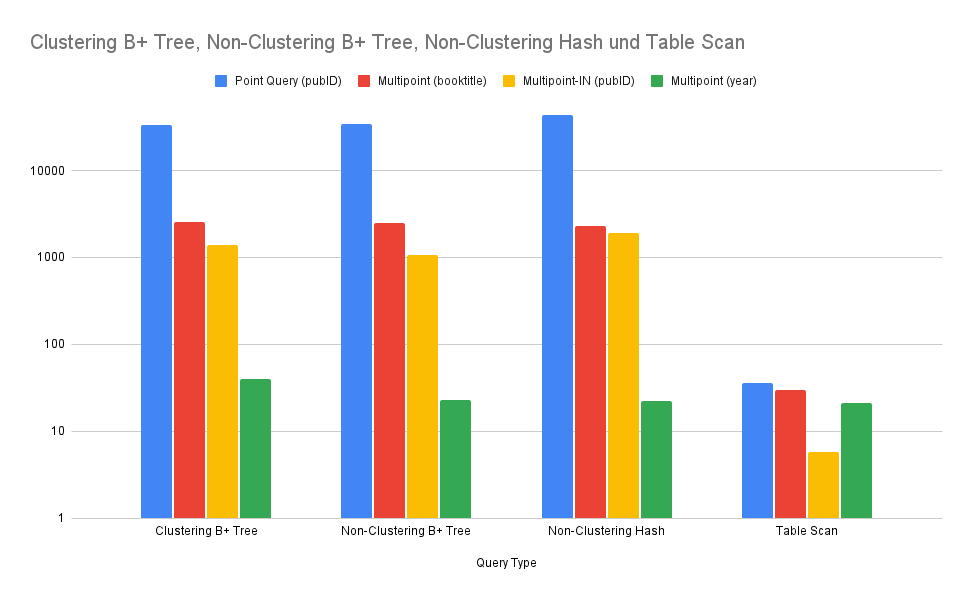
\includegraphics[width=\textwidth]{resources/throughput.png}

Firstly, we will look at the point query.
The clustering and non-clustering B$^+$ tree indexes have a similar throughput.
The non-clustering hash index has the highest throughput, which is expected, as hash indexes are faster for point queries.
As Expected, the table scan has the lowest throughput, as there is no index that can be used.

Regarding the multipoint query with low selectivity, the B$^+$ indexes and the hash index performed somewhat similarly.
The clustering B$^+$ index had the highest throughput, which makes sense since the clustering index sorts the data
by the indexed attribute, which benefits ranged queries.
Again, the table scan had the lowest throughput.

For the multipoint query with the IN-Predicate, the Hash index outperformed the B$^+$ indexes.
This outcome is quite interesting; from a naive perspective, one would expect the clustered B$^+$ index to perform
better than the hash index.
However, since there are multiple exact mathes involved in the IN-Predicate, the hash index is faster.
And just like with the previous queries, the table scan had the lowest throughput.

Lastly, for the multipoint query with high selectivity, the clustering B$^+$ index had the highest throughput, having
almost double the throughput of all the other methods.
This is expected, as the sorting of the data helps a lot with this type of query.
The rest performed similarly, but the table scan still had the lowest throughput.



\subsection*{Time Spent on this Assignment}

Time in hours per person: \textbf{XXX}

\subsection*{References}

\printbibliography

\end{document}
